\documentclass[12pt, UTF8]{article}
\usepackage[a4paper, scale = 0.8]{geometry}
\usepackage{ctex}

\usepackage{listings}
\usepackage{xcolor}
\usepackage{fontspec}
\usepackage{sourcecodepro}
\lstset{
  keywordstyle = \color{blue!70},
  commentstyle = \color{green!70!blue!70},
  rulesepcolor = \color{red!20!green!20!blue!20},
  basicstyle = \ttfamily,
  backgroundcolor = \color[RGB]{245,245,244},
  breaklines=true,
}

\usepackage{graphicx}
\usepackage{amsmath}

\usepackage[colorlinks, linkcolor = red, anchorcolor = blue, citecolor = green]{hyperref}

\renewcommand\thesection{\arabic{section}}

\title{数据挖掘第二次作业}
\author{李晨昊 2017011466}
\begin{document}
\maketitle
\tableofcontents

\section{数据属性类型练习}

\begin{itemize}
  \item 教师的职称:Ordinal,职称是一组离散的值,且可以比较大小(职称有高低之分)
  \item 手机号码:Nominal,手机号码是一组离散的值,且无法比较大小(其大小关系无意义),也不能运算
  \item 体重:Ratio,体重可以进行各种运算
  \item 出生日期:Ordinal,出生日期是一组离散的值,且可以比较大小
  \item 出生地:Nominal,出生地是一组离散的值,且无法比较大小,也不能运算
  \item 年龄:Interval,年龄的乘除运算无意义(或者说实际中很少用到)
\end{itemize}

\section{计算统计信息}

\begin{enumerate}
  \item
    \begin{itemize}
      \item 均值:28.01875
      \item 中位数:28.1
      \item 众数:26.5
    \end{itemize}
  \item
    \begin{itemize}
      \item 最小值:7.8
      \item 第一四分位数:26.5
      \item 中位数:28.1
      \item 第三四分位数:33.575
      \item 最大值:43.0
    \end{itemize}
    
    盒图见\ref{fig:box}。
    
    \begin{figure}[!ht]
      \centering
      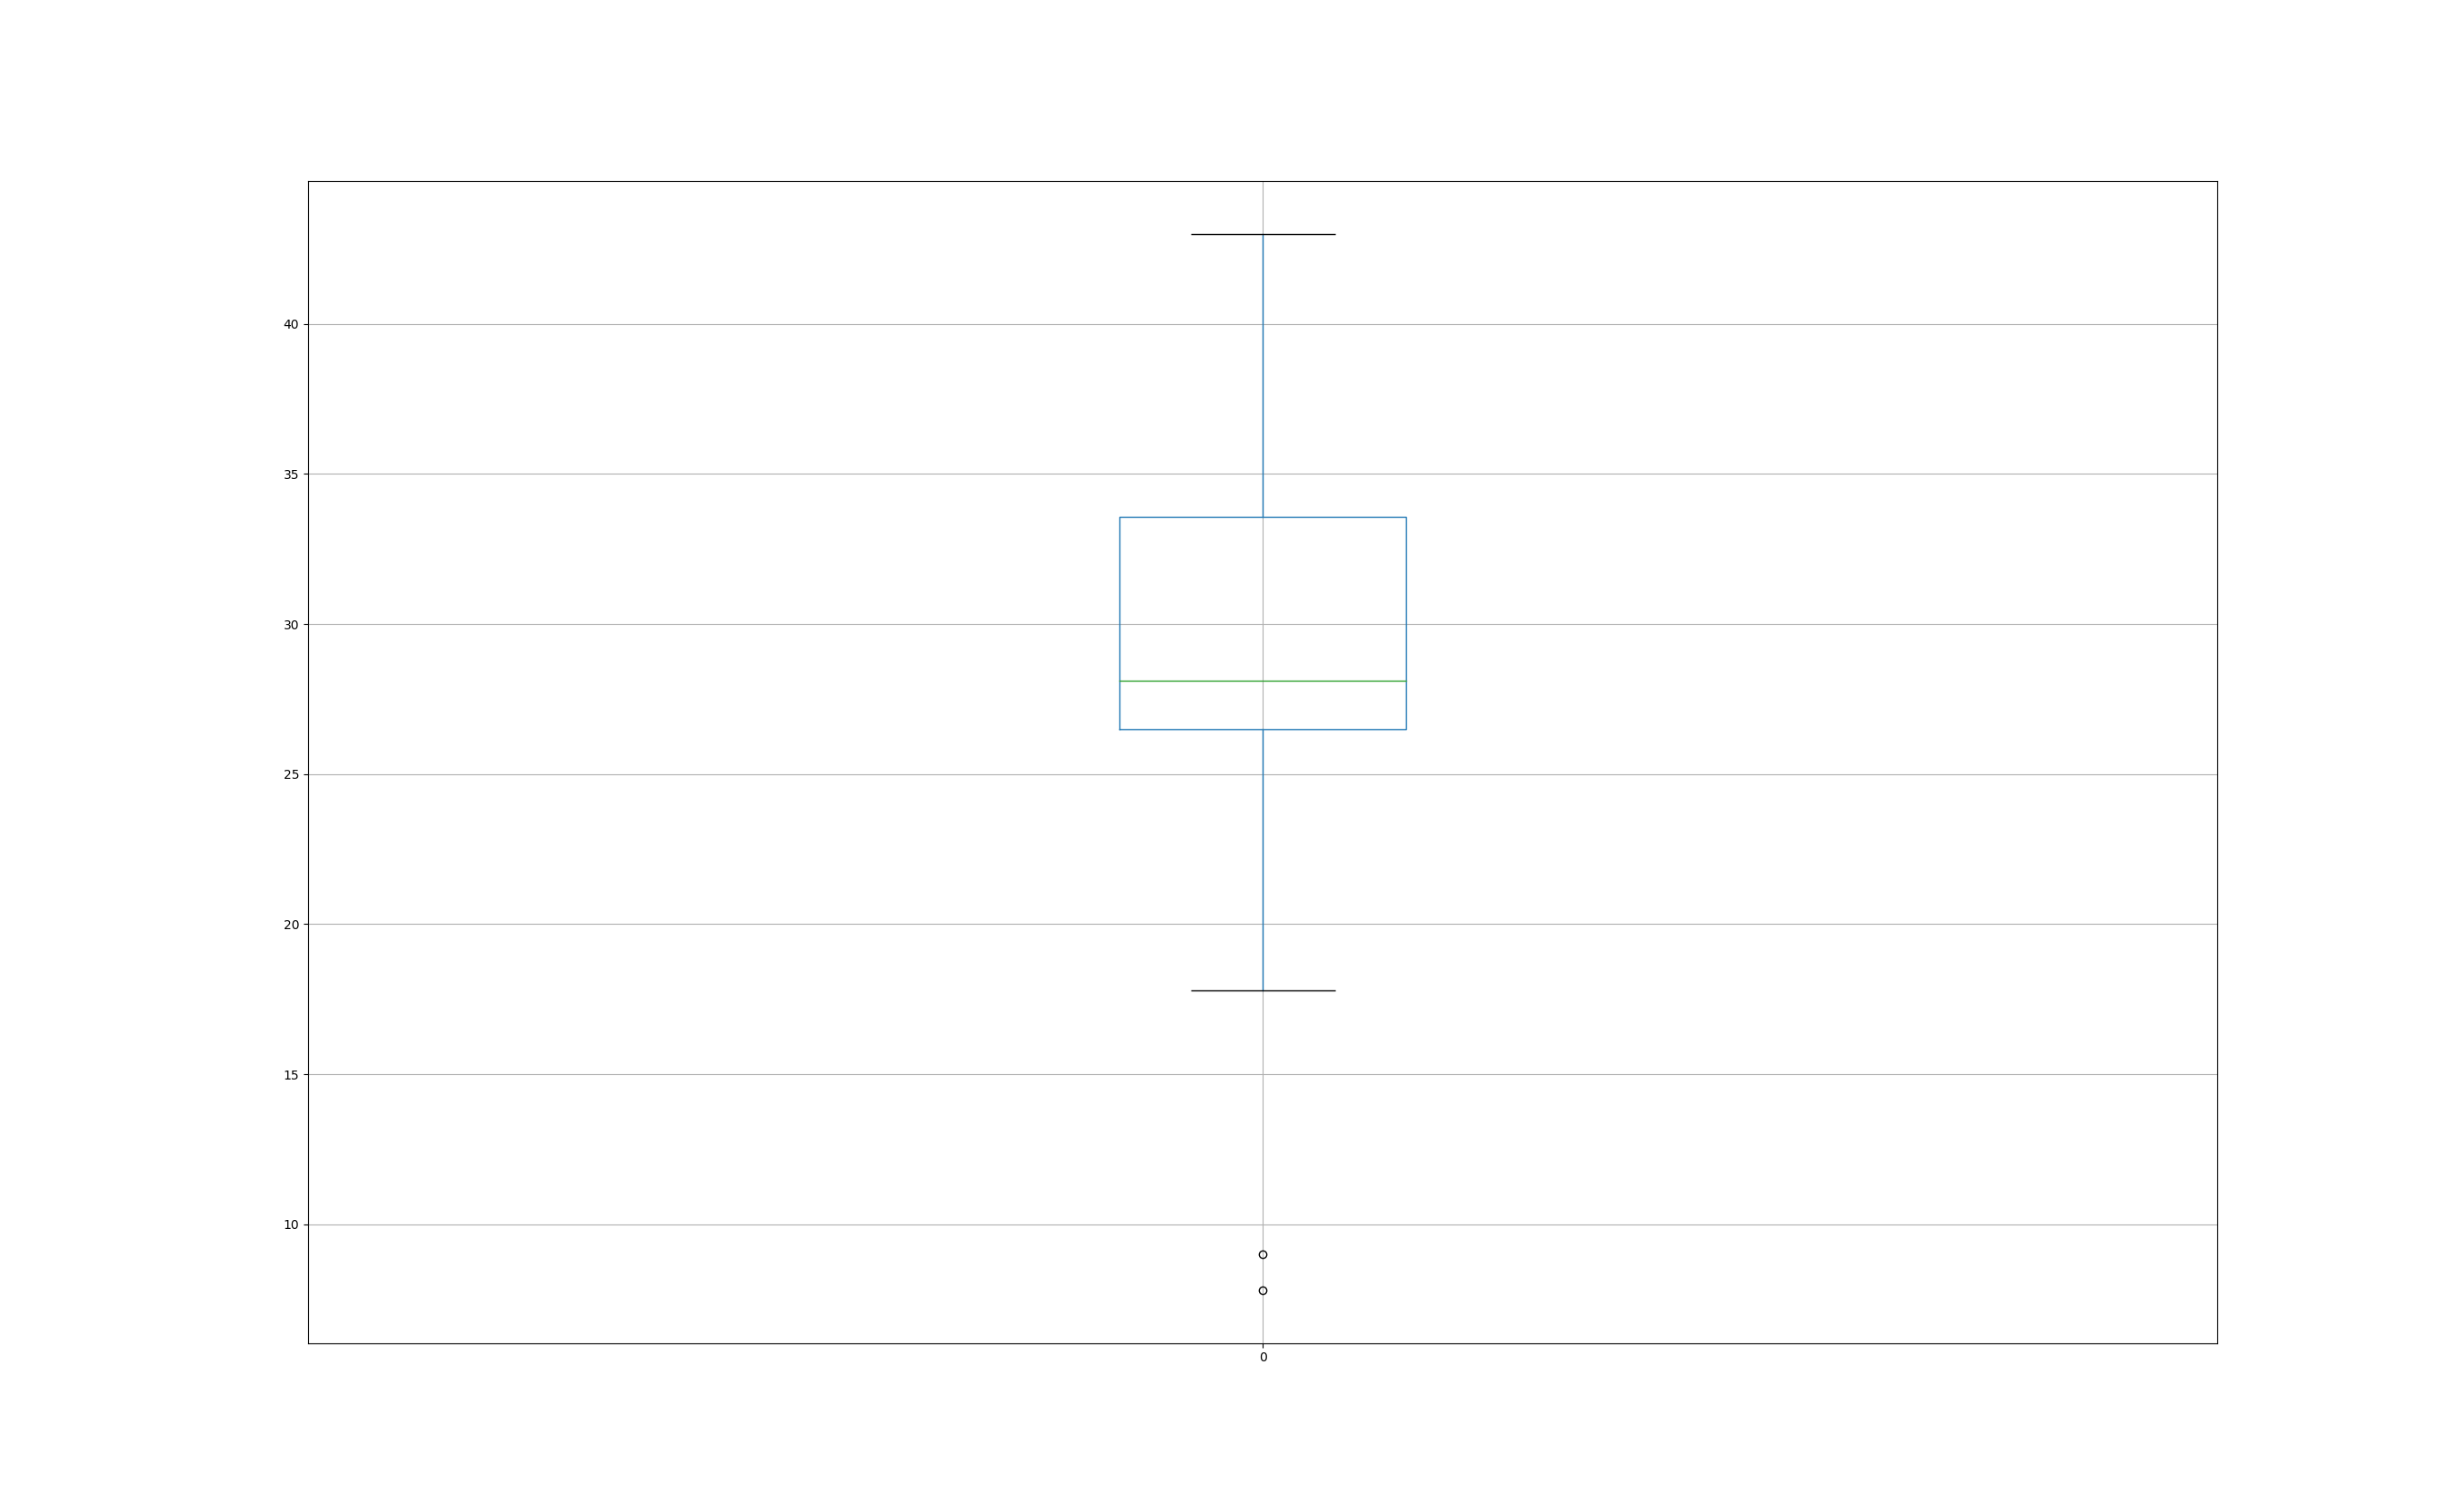
\includegraphics[width=1.0\textwidth]{box.png}
      \caption{盒图}
      \label{fig:box}
    \end{figure}
\end{enumerate}

\section{文本数据的表示}

我使用Rust完成本实验,代码和数据都附在了提交的doc文件夹中,在该文件夹中执行\lstinline{cargo run --release}即可运行程序。

\subsection{实现思路}

\subsubsection{词典构造}

首先读入每个文件的全部内容,存储在一个\lstinline{Vec<String>}中,这样后续使用的字符串来自其中的引用,可以减少复制的开销。

接着为每个文件建立词典,方法是先删除所有除了字母,数字和空格的内容,即删除标点符号,然后按照空格分词,然后把这些字符串插入散列表中,同时维护计数。

与此同时,构建全局的词典和共现矩阵,方法都是平凡的。共现矩阵定义为\lstinline{HashMap<&str, HashMap<&str, u32>>},其中可以考虑每个词和自身的共现,也可以不考虑,经测试结果基本没有区别,所以我选择了考虑,这样编写简单一些。

在建立了全局的词典之后修改每个文件的词典,依据每个词的计数值计算出tf-idf值。

\subsubsection{距离计算}

文件相似度通过每个文件的词典来计算。将每个文件的词典的列表按照距离来排序,选择前几个即可。排序通过Rust提供的\lstinline|sort_by_cached_key|,这样可以避免重复计算。Euclidean距离的计算通过枚举给定文件的词,将其tf-idf值与目标文件对应词的tf-idf值(若这个词不存在则取0)相减,平方,再求和;再加上目标文件中不在给定文件中的词的tf-idf值的平方和。结果不需要开根号,因为只是为了比较大小。

Cosine距离的计算通过枚举给定文件的词,将其tf-idf值与目标文件对应词的tf-idf值(若这个词不存在则取0)相乘,再求和,得到向量点乘的值;再除以两个文件中各自所有词tf-idf值的平方和的积的平方根,得到$\cos(\text{向量夹角})$,这个值与向量间的相似程度成正相关,因此对它取负,再排序,这样前几个元素就是相似程度最高的。

词语相关度通过共现矩阵来计算。计算方式与上面类似,不再重复。

\subsection{结果与分析}

运行程序得到如下输出:

\begin{lstlisting}
doc similarity with doc 52
by euclidean distance: [31, 256, 258, 194, 212]
by cosine distance: [31, 258, 256, 194, 97]
word similarity with word "crime"
by euclidean distance: ["trial", "college", "Sebastian", "Randy", "revealed"]
by cosine distance: ["trial", "college", "lawyer", "say", "Sebastian"]
\end{lstlisting}

其中分析了与名称为52的文章相似的文章和与词crime相关的词。这两个值都是随意取的,可以通过修改代码来替换成别的值。

文章部分,文章52看起来像是节目预告或者新闻之类的文章,其中依据时间记录了一系列事实,许多事实与犯罪相关。文章31是完全类似的,所以两种方法都把它排在第一位。还有几个前几名的文章也是类似的,还有几个文章只是记录犯罪内容的,相关度较低一些,也排在前几名。

词语部分,找到的trial显然与crime关系很大,还有lawyer的关系也比较大。其他词的关系看起来没那么大,可能是人名或者地名,猜测也许在几篇记录犯罪的文章中都出现了它们。

\end{document}

